\documentclass{beamer}

\usepackage{graphicx} % For including images
\usepackage{hyperref} % For including links
\usepackage{amsmath}  % For mathematical symbols
\usepackage{listings} % For code snippets

% Theme for Beamer
\usetheme{Madrid}

% Title of the presentation
\title[Capstone Project]{Data Science Capstone Project}
\subtitle{A detailed technical report on the data science journey}
\author{Eid Alkhaldi}
\date{\today}

% Start of the document
\begin{document}

% Title slide
\begin{frame}
    \titlepage
\end{frame}

% Executive Summary
\section{Executive Summary}
\begin{frame}{Executive Summary}
    \begin{itemize}
        \item Briefly outline the project goals, key findings, and conclusions.
        \item Summarize the outcomes of the project, such as predictive analysis results and innovative insights.
        \item Highlight key technical milestones achieved.
    \end{itemize}
\end{frame}

% Introduction
\section{Introduction}
\begin{frame}{Introduction}
    \begin{itemize}
        \item Provide an overview of the problem statement and objectives of the project.
        \item Introduce the methodology and technologies used (e.g., Python, SQL, EDA, Folium, Plotly Dash).
        \item Explain the structure of the presentation and how each section relates to the overall project.
    \end{itemize}
\end{frame}

% Data Collection and Wrangling
\section{Data Collection \& Wrangling}
\begin{frame}{Data Collection and Wrangling Methodology}
    \begin{itemize}
        \item Detail the data sources and the process of gathering the data.
        \item Explain the data wrangling techniques used to clean and prepare the dataset.
        \item Include code snippets or images if applicable.
    \end{itemize}
    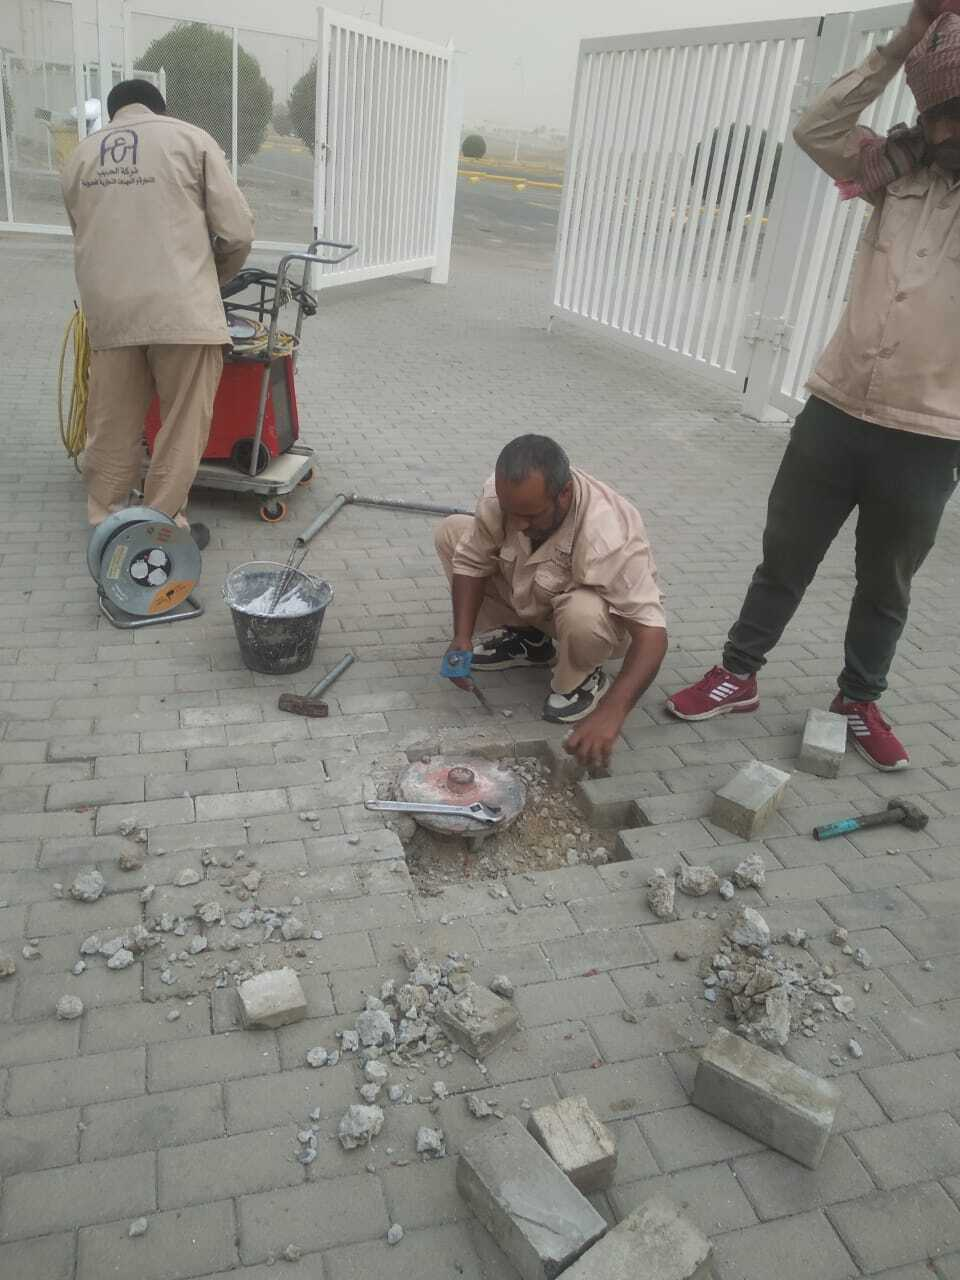
\includegraphics[width=0.8\textwidth]{images/data_wrangling.jpg}
\end{frame}

% Exploratory Data Analysis (EDA) - Methodology
\section{EDA and Visual Analytics}
\begin{frame}{Exploratory Data Analysis Methodology}
    \begin{itemize}
        \item Describe the exploratory data analysis process.
        \item Discuss the tools and libraries used (e.g., Pandas, Matplotlib, Seaborn).
        \item Explain how interactive visual analytics were conducted.
    \end{itemize}
\end{frame}

% EDA Results with Visualization
\section{EDA Results with Visualizations}
\begin{frame}{Exploratory Data Analysis Results}
    \begin{itemize}
        \item Show key insights found during EDA.
        \item Use visualizations to represent data distributions, correlations, etc.
    \end{itemize}
    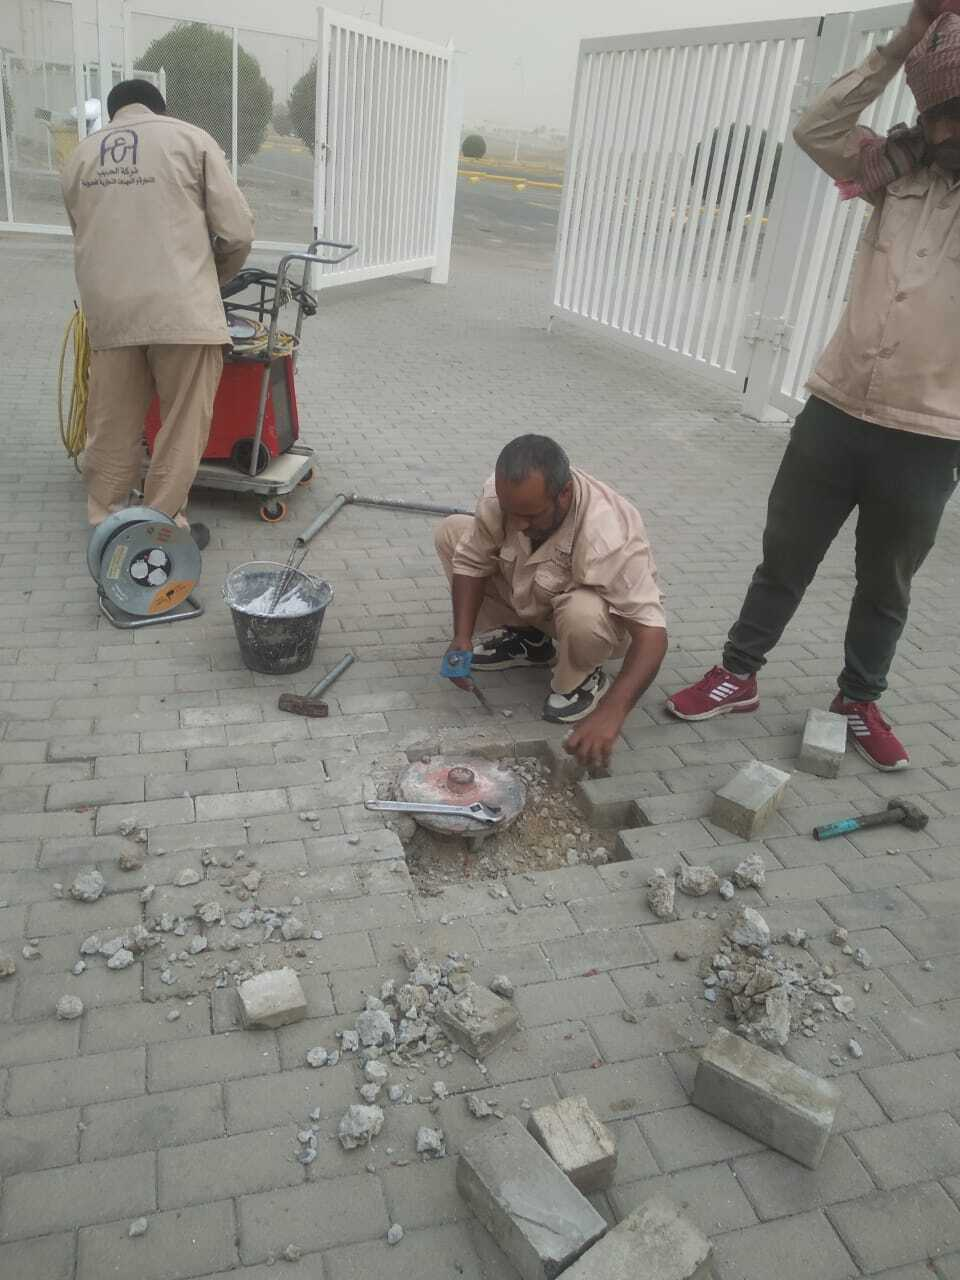
\includegraphics[width=0.8\textwidth]{images/eda_results.jpg}
\end{frame}

% EDA Results with SQL
\section{EDA with SQL Results}
\begin{frame}{EDA with SQL Results}
    \begin{itemize}
        \item Discuss the use of SQL queries to extract insights from the data.
        \item Include examples of SQL queries and their results.
    \end{itemize}
    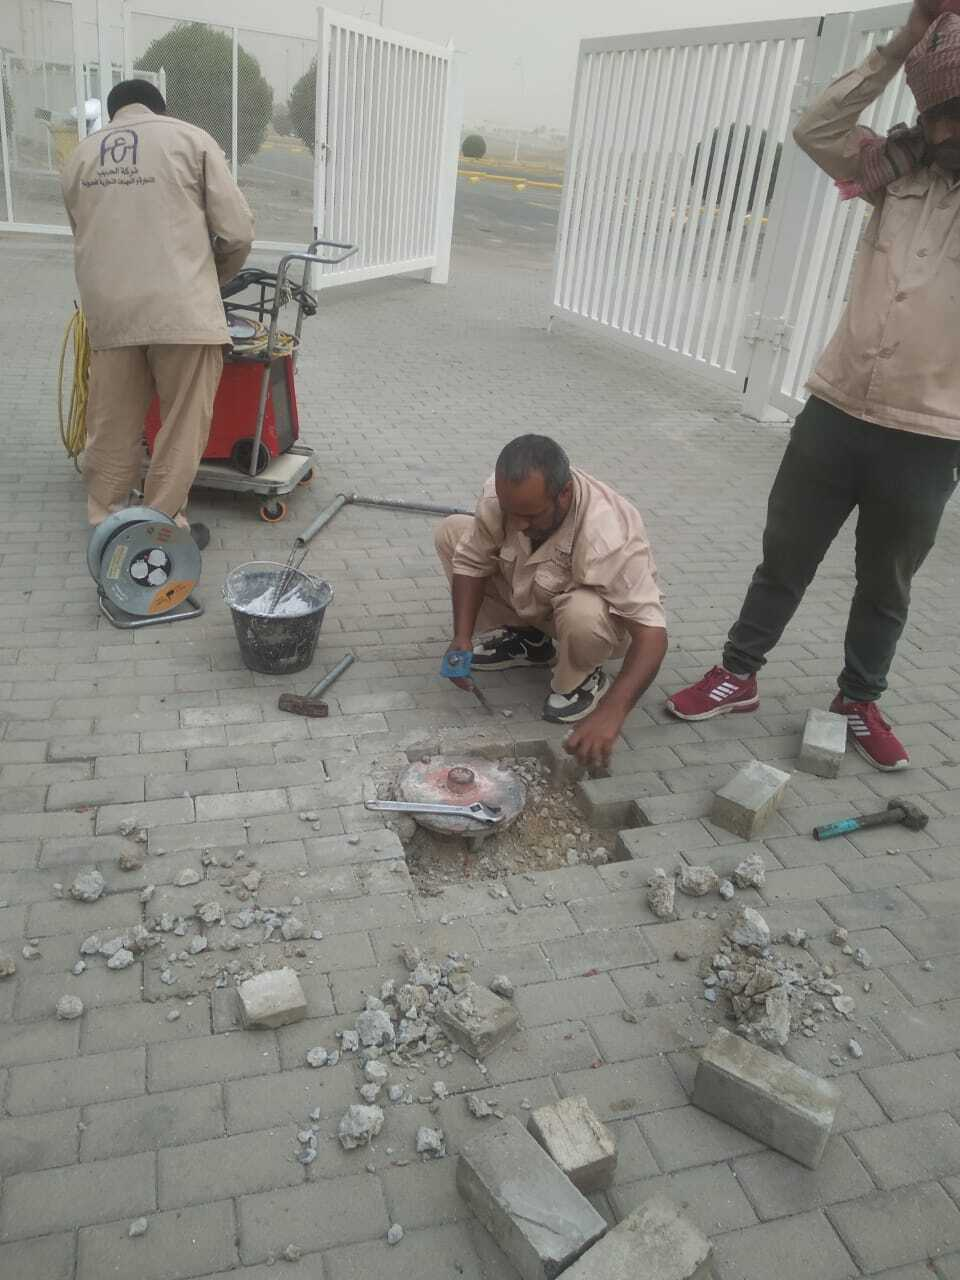
\includegraphics[width=0.8\textwidth]{images/sql_results.jpg}
\end{frame}

% Interactive Map with Folium
\section{Interactive Map}
\begin{frame}{Interactive Map with Folium}
    \begin{itemize}
        \item Explain the creation of an interactive map using Folium.
        \item Show screenshots or embed code snippets to demonstrate map functionality.
    \end{itemize}
    \includegraphics[width=0.8\textwidth]{images/folium_map.jpg}
\end{frame}

% Dashboard with Plotly Dash
\section{Plotly Dash Dashboard}
\begin{frame}{Interactive Dashboard with Plotly Dash}
    \begin{itemize}
        \item Discuss how the dashboard was built using Plotly Dash.
        \item Highlight key features and the insights derived from the dashboard.
    \end{itemize}
    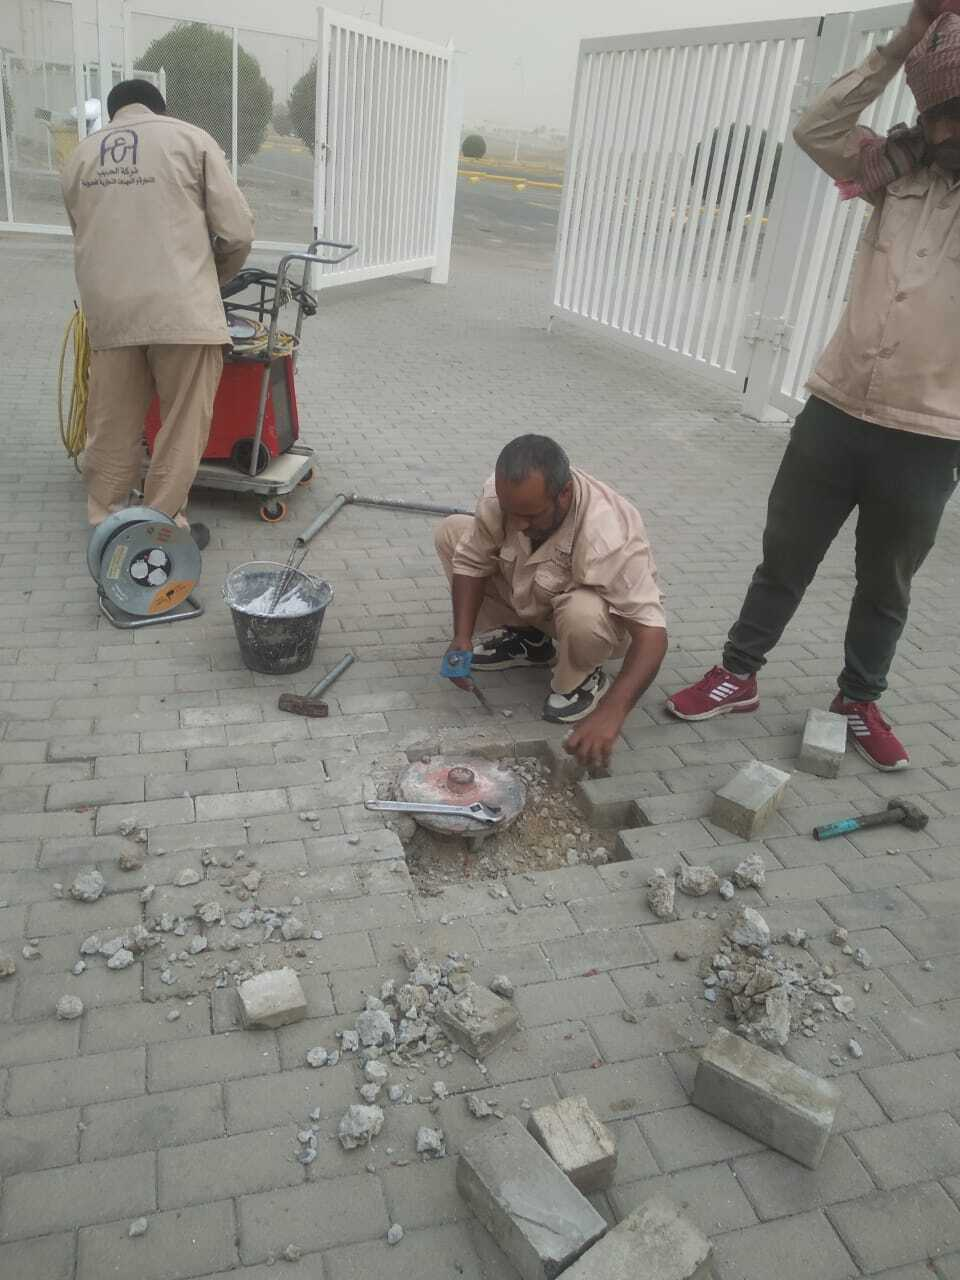
\includegraphics[width=0.8\textwidth]{images/plotly_dashboard.jpg}
\end{frame}

% Predictive Analysis Methodology
\section{Predictive Analysis}
\begin{frame}{Predictive Analysis Methodology}
    \begin{itemize}
        \item Detail the methodology used for predictive analysis (e.g., classification techniques).
        \item Explain the steps taken to train, validate, and test the model.
        \item Mention any hyperparameter tuning or model selection techniques.
    \end{itemize}
\end{frame}

% Predictive Analysis Results
\begin{frame}{Predictive Analysis Results}
    \begin{itemize}
        \item Present the classification results, including accuracy, precision, and recall.
        \item Include charts or confusion matrices to represent the model's performance.
    \end{itemize}
    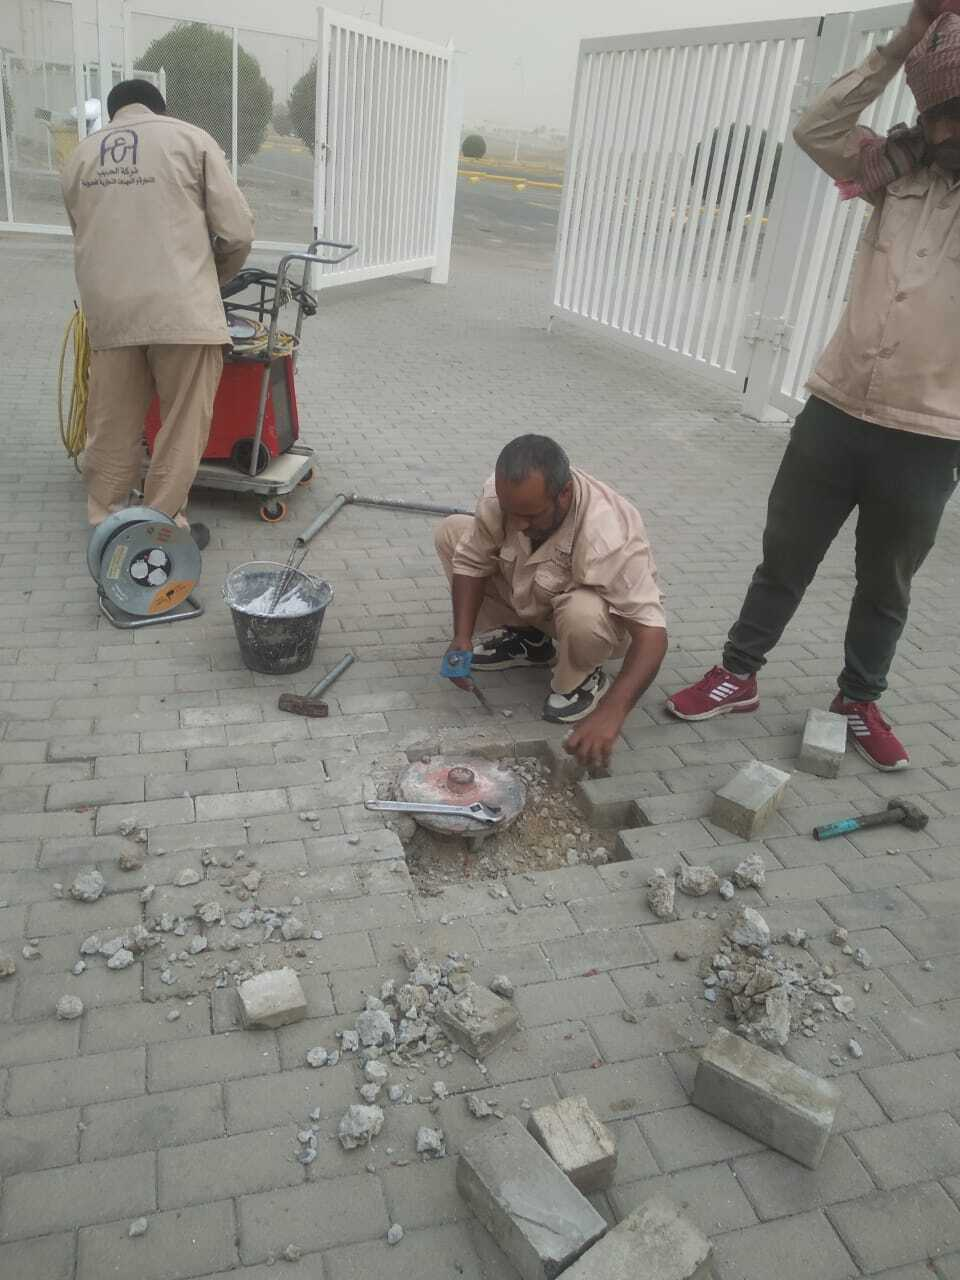
\includegraphics[width=0.8\textwidth]{images/predictive_results.jpg}
\end{frame}

% Conclusion
\section{Conclusion}
\begin{frame}{Conclusion}
    \begin{itemize}
        \item Summarize the outcomes of the project.
        \item Highlight key technical achievements and insights.
        \item Discuss potential next steps and improvements.
    \end{itemize}
\end{frame}

% Creativity and Innovation (Optional slide)
\section{Creativity and Innovation}
\begin{frame}{Creativity and Innovative Insights}
    \begin{itemize}
        \item Highlight any innovative techniques or tools you applied beyond the template.
        \item Discuss any unique insights or approaches that added value to the project.
    \end{itemize}
\end{frame}

% End of the presentation
\end{document}
